\documentclass[conference]{IEEEtran}
\usepackage{cite}
\usepackage{amsmath,amssymb,amsfonts}
\usepackage{algorithmic}
\usepackage{textcomp}
\usepackage{xcolor}
\usepackage{float}
\usepackage[T1]{fontenc}
\usepackage{graphicx}
\usepackage{listings}
\usepackage[utf8]{inputenc}
\usepackage[backend=biber, sorting=none]{biblatex}
\addbibresource{bibliography-biblatex.bib}
\usepackage[paperheight=27.94cm,paperwidth=21.59cm,left=2.54cm,right=2.54cm,top=2.54cm,bottom=2.54cm]{geometry}
\lstset{numbers=left,
  inputencoding=latin1,
  basicstyle=\footnotesize\ttfamily,
  keywordstyle=\color{blue},         
  breaklines=true, 
  showtabs=false,
  showstringspaces=false,
  numberstyle=\tiny\color{mygray}
}

\setlength\parindent{0pt}
\renewcommand{\arraystretch}{1.3}

\title{Sudoku Solver}
\begin{document}

\author{\IEEEauthorblockN{Exdol Davy}
\IEEEauthorblockA{\textit{Undergraduate, Dept. Comp Sci.} \\
\textit{University of Central Florida}\\
Orlando, FL, USA \\
exdoldavy@knights.ucf.edu}
\and
\IEEEauthorblockN{Douglas Glover}
\IEEEauthorblockA{\textit{Undergraduate, Dept. Comp Sci.} \\
\textit{University of Central Florida}\\
Orlando, FL, USA \\
douglasglover3@knights.ucf.edu}
\and
\IEEEauthorblockN{Kashyap Rana}
\IEEEauthorblockA{\textit{Undergraduate, Dept. Comp Sci.} \\
\textit{University of Central Florida}\\
Orlando, FL, USA \\
kashyap\textunderscore rana@knights.ucf.edu}
\and
\IEEEauthorblockN{Matthew Singh}
\IEEEauthorblockA{\textit{Undergraduate, Dept. Comp Sci.} \\
\textit{University of Central Florida}\\
Orlando, FL, USA \\
mattsingh@knights.ucf.edu}
\and
\IEEEauthorblockN{Miguel Venero}
\IEEEauthorblockA{\textit{Undergraduate, Dept. Comp Sci.} \\
\textit{University of Central Florida}\\
Orlando, FL, USA \\
venero@knights.ucf.edu}
}
\maketitle

\vspace{2\baselineskip}


\vspace{1\baselineskip}

\begin{abstract}
Malformed Sudoku puzzles (or Sudoku puzzles that have more than one solution) are an unlikely occurrence in today's world of computers, as opposed to when Sudoku puzzles were created only by man. However, they are not impossible to be produced accidentally (or even on purpose). It has been mathematically proven by Gary McGuire, Bastian Tugemann, and Gilles Civario in 2012 [1] that a Sudoku puzzle must provide at least 17 valid clues to contain exactly 1 unique solution. This project will provide further analysis upon this proof, while determining whether a Sudoku puzzle can be solved or not.
\end{abstract}

\vspace{1\baselineskip}

\section{Introduction}
Sudoku is a Japanese puzzle game that requires players to fill all of eighty-one boxes presented in a 9x9 grid. The content of each box must be any integer between the interval of 1 through 9 inclusively. The 9x9 grid is also divided into nine blocks (with three blocks being in each row and three blocks being in each column), each of which contain nine boxes, therefore also being a 3x3 grid. The image below is an example of the 9x9 grid, with all nine of the 3x3 grid blocks.

\vspace{1\baselineskip}
\begin{figure}[H]
\centering
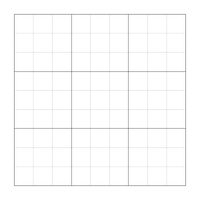
\includegraphics[width=5.11cm,height=4.87cm]{sudokujpg.jpg}
\end{figure}

\vspace{1\baselineskip}
Each Sudoku puzzle typically starts off with at least seventeen clues to be guaranteed to have a valid solution, but can contain more depending on the difficulty level. However, to successfully complete the game, the player must fill all empty boxes, in the 9x9 grid, such that each of the nine blocks contain exactly nine integers from the interval of 1 through 9 inclusive without repetition (each integer being within its own respective box). In addition to this, the boxes within each column and each row of the 9x9 grid must contain an integer from the interval of 1 through 9 inclusive without any duplicates being in each column and row respectively. 

\vspace{1\baselineskip}

\section{Problem Statement}
The most simple way to solve a Sudoku puzzle would be to try all the nine possible numbers in all eighty-one boxes. If a digit does not violate any of the Sudoku rules (i.e., if it does not appear in the same row, column, or sub-grid), it is placed in the cell, and the process is repeated for the next empty cell. If a digit violates the rules, it is discarded, and the next digit is tried until a valid solution is found. This approach for Solving Sudoku puzzles involves exhaustively testing all possible solutions to find the correct one which is slow and inefficient. The ability to efficiently determine whether a puzzle is solvable or has multiple solutions is important for studying the complexity of Sudoku problems. We will explore the different methods and techniques used to solve Sudoku puzzles, evaluate their effectiveness and efficiency, and identify the challenges and limitations associated with each method. Also implement multi threading to see if it actually benefits the run time or is not effective at all.

\section{Related Work}
Gary McGuire of University College Dublin published a proof which claims that the minimum number of clues needed to solve a Sudoku puzzle is seventeen. The abstract of the work mentioned the hitting set problem being computationally hard; it is one of Karp’s 21 classic NP-complete problems. The study mentioned that standard backtracking algorithm for finding hitting sets would not be fast enough to search for a 16-clue Sudoku puzzle exhaustively. They had to design an algorithm that efficiently enumerated hitting sets of a suitable size. Then they later claimed "There Is No 16-Clue Sudoku"[1].


\section{Methodology - Pen \& Paper Approach}
To better understand how to systematically solve a sudoku, we first created a single thread implementation of solving sudoku
which was a brute force method where it checks all possible values for each cell and iterates until the grid has been solved.
\\*

The next step was to come up with a multithreading approach for the problem. At first we thought to have two threads, one for the
column and one for the row, then both would work together to find all possible options for each cell to solve the sudoku.
This method does not properly use multithreading concepts to their full potential as it takes the single thread approach and assigns
threads to specific assignments. We decided that we did not want our project to move in this direction so we halted the
implementation of this approach.
\\*

After some discussions on what multithreading approaches we should take, more research was conducted.
To properly solve a grid we dived into understanding how average humans go about solving the sudoku, the pencil and paper algorithm.
A human uses the clues provided by the given numbers in the grid and uses logic to determine which values must
exist in particular cells. One of the most common strategies is to use the process of elimination, finding all the values that
are impossible in a cell. If there is only one value that remains possible, we know that it is the correct value.
\\*

The best way to combine common sudoku-solving strategies with multithreading was to first split the grid into pieces.
Assume we are working with a classic 9x9 sudoku grid. Each thread is to be given a row, column, and box (3x3 cell group).
This will split the grid evenly across nine separate threads. Each thread shares access to a three-dimensional matrix of boolean values
(9x9x9). The first two dimensions refer to a specific cell’s location in the grid, and the last dimension is used to track
which of the possible numbers for that cell have been eliminated.
\\*

This allows threads to share information on the values deemed impossible for each cell.
If all possible values in a cell are eliminated except for one, then the thread will mark it as the correct value for that cell.
\\*

There are four strategies that the program uses to determine the solution:
\vspace{1\baselineskip}
\begin{itemize}
    \item{If a number has been used in a row, column, or box, 
    then that number should be marked as impossible for all other cells in that row, column, or box.}

    \item{If a cell has all numbers deemed impossible except for one, 
    then that last number is the correct value for the cell.}

    \item{If a cell is the only cell in a row, column, or box where a number is possible, 
    then that number is the correct number for the cell.}

    \item{If there exists some number that must exist in both a specific row and box or a specific column and box, 
    then that number should be marked as impossible for any cells in the box outside the specific row or column.}
\end{itemize}
Using these four strategies allows the puzzle to be solved in a step-by-step method similar to how a person might solve it.

\section{Methodology - BFS Memoization Approach}
The main issue with the DFS/backtracking implementation of solving Sudoku puzzles is that it complicates many viable incorporation of threads. Since, the method that is tasked with solving the puzzle in a brute force way incorporates recursion, we could not simply send the next method into a thread. If we were to do this, the program would promote functionality that leads to seemingly infinite thread creation. This occurs when a thread currently performing the method, gets to the recursive call that sends the method to another thread. Hypothetically, if that were to happen, the main thread would not halt until the thread it called has halted, creating a chain of longer-living and redundant threads, thus establishing immensely inefficient thread creation; and the number of threads must be stable to ensure proper balancing of work. Despite this, our DFS single threaded brute force approach is a great baseline for comparisons to other approaches, especially others that also incorporate brute force such as the BFS Memoization Implementation.
\\*

During the process of creating the BFS Memoization Implementation, we first created a single threaded approach. This approach had two global variables, a HashMap (puzzleStates) and a HashSet (solutionHashes).
\\*

We simulate a Breadth First Search by receiving all possible moves or states from each currently filled out puzzle (starting from filling the top left first and through the puzzle to the bottom right). The solve(String startGridHash) creates a queue of each iteration's breadth or work that can be further worked on using the getNext(String currentPuzzleHash) method; the solve method also checks each puzzle in the queue for completion, but to ensure efficiency, it only does that check if the puzzleStates value - that is accessed in O(1) - implies completion (row value was incremented to the end) since the completion check is O(n). The puzzleStates HashMap’s memoized puzzle state is both accessed and manipulated in the getNext method, which is called until the queue of all puzzle states is empty (which means that they have either been removed from being invalid or removed from being a solution).
\\*
Lastly, we can multithread our approach by establishing a shared queue among multiple threads that will retrieve from contribute to the aforementioned queue. These threads are joined so that they all must be done working prior to our program checking if solutions are available.
\\*

\subsection{puzzleStates}
The purpose of the puzzleStates HashMap was to hold all possible (or at least, all previously visited) puzzle states or combinations that build upon the hints already given and most times with the work already done by previous iterations. The key of this HashMap held a String that would be concatenated with all the integers in the 81 boxes at the same time; we used the number zero to represent empty boxes that haven’t yet been filled by our program. An example of this would be the string “53007000060019500009800006080006000340080300-
\\*
1700020006060000280000419005000080079” for the starting state of a puzzle with one solution. For better visual understanding, it is important to note that in the code, the puzzle would be represented in a 2D array like this:
\vspace{1\baselineskip}
\begin{figure}[H]
\centering
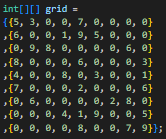
\includegraphics[width=5.11cm,height=4.87cm]{one_solution_puzzle.png}
\end{figure}

We can create strings like this by looping through each row and column from top left to bottom right of the puzzle and concatenating that value to an initial string of “” (empty string). We can turn these strings back into a 2D array, by looping through each character of the string in 9 loops of 9 loops (81 iterations total) and setting that specific row and col in the grid to be what that character currently is from the string. A better way to explain this would be that the column (or 1st index and inner/nested loop) is going to be the remainder of the current index of the string divided by 9. 
\\*

\begin{itemize}
\item The index of the first 7 in the string for this starting puzzle would be 4 so 4%9 = 4, the first 6 is at index 9 so 9%9 = 0, thus their column indexes are 4 and 0 respectively
\end{itemize}
Additionally, the row (or 0th index and outer loop) can be described as the floor of the current index of the string divided by 9.
\begin{itemize}
\item Using our previous example’s numbers, the index of the first 7 in the string for this starting puzzle would be 4 so floor(4/9) = 0, the first 6 is at index 9 so floor(9/9) = 1, thus their row indices are 0 and 1 respectively.
\item In full, the coordinates of the first 7 and the first 6 would be (0,4) and (1,0) respectively. If the program were to have filled out all of the zeroes in the puzzle preceding 7 and 6, respectively, with all possible valid numbers, their coordinates/location in the puzzle would be the values of their puzzle’s state’s hashed string key, establishing that those numbers are the next to be checked if they can hold different numbers (which they can’t because they are non-zero, but the program realizes this in itself).
\end{itemize}
Moreover, the value of this key in the HashMap would be an ArrayList  of type Integer that holds at most and at least two values. These values represent the current position of the program after it has made one move (or filled in one additional square). The two values represent the row and column of the next move/decision to be made by the next breadth or iteration (both intervals are [0, 8] since it is a 9x9 2D array and Java indexes use zero-based numbering). In our previous example (of the one solution starting puzzle), that key’s corresponding value would be [0, 0]. When a puzzle state is updated, its value’s 1 indexed element is positively incremented by 1 unless it is at 8, otherwise it will change to 0 and positively increment the 0 indexed element by 1. Once the 0 indexed element is greater than 8, this puzzle is detected by our program and validated to be a solution; once that is done, its key value from the HashMap is added to our solutionHashes Hashset.
\subsection{solutionHashes}
The sole purpose of the solutionHashes HashSet is to store the states of all finished and valid puzzles. The usefulness in using a HashSet is that if another iteration of our program finds the same puzzle state as a solution and attempts to add it to the solutionHashes HashSet, it will not create a duplicate. However, the problem and our program prevents this from happening since the puzzleStates HashMap already avoids duplicate keys. HashSets are also dynamic in nature and have a time complexity of O(1) of both insertion retrieval. We can also use the size of the solutionHashes HashSet to get the current and total count of solutions solved by our program. If solutionHashes.size() == 0, then there were no solutions, if solutionHashes.size() == 1, then there was one solution, and if solutionHashes.size() > 1, then there were more than one solution.
\subsection{solve}
The solve method is called with the parameter of the concatenated string created with the initial sudoku puzzle. When it begins, it creates a queue in the form of a LinkedList that holds Strings and adds only the singular and initial concatenated string. The rest of the method is a while loop that continues only if the queue is not empty (queue.size() != 0). It is also important to note that this method has no return type and is void, because every solution will already be in the solutionHashes HashSet by the time the program is near termination.
\\*

In the while loop of this method, we dequeue the queue to get a given puzzle state. In each loop, the puzzle state dequeue tends to build up from previous puzzle states since they are added back to the queue if they are not done yet and each step is one breadth/iteration towards completion. After the dequeue, a series of next possible breadths/iterations are retrieved by the getNext method in the form of an ArrayList of Strings. This ArrayList holds concatenated puzzle states that build off of the passed concatenated puzzle state. The rest of the while loop is a loop through this ArrayList.
\\*

In the looping of the ArrayList, each String is checked if its value’s 0th indexed element is greater than 8 or not (accessed through the puzzleState HashMap). If it's greater than 8, then it is checked if it is complete with the isComplete method which returns false if any zeroes exist within the string it is passed or true, otherwise; this String then gets added to the solutionHashesHashSet. If the value’s 0th indexed element is less than or equal to 8, it is added back to the queue as is.
\\*

\subsection{getNext}
The getNext method is passed any puzzle hash (that already exists in the puzzleStates HashMap) and returns an ArrayList of Strings (that represent the possible puzzle hashes of puzzle states 1 move ahead of the puzzle that was passed to the method). There is first a check of whether the current position of the puzzle holds a 0 or not. If a 0 is not at the current position of the puzzle, it will increment the position, store that new position in the puzzleStates HashMap, then return an ArrayList holding the same puzzle state it was initially passed. If a 0 is at the current position of the puzzle, the method will increment a temporary variable holding the next position, try all valid numbers at the current position, concatenate the puzzle with that number at the current position, and place into the puzzleStates HashMap both that new puzzle state and the incremented temporary variable holding the next position. Lastly, those new states are added to the ArrayList of Strings that will be returned by this method. After the if statement logic is finished, the ArrayList of Strings is returned.
\\*

\subsection{Implementing Multi-Threading}
We constructed a multithreaded implementation using this approach by converting the solve method to initialize our threads with the pointer to our queue (to be shared among all threads) and starting them there. We also converted the queue into a LinkedBlockingQueue that is thread-safe. Each thread will then run the while loop that previously existed within the solve method. The threads will then contribute to the queue as needed and are joined in the solve method to end at the same time. In both before and after the multithreading implementation, the queue starts small and reaches around 700 in size near the middle of the program, then approaches 0 at the end.
\\*
\begin{lstlisting}[language=Java,numbers=none]
public Queue<String> queue;

public SudokuSolverMultiBFSMemo(Queue<String> queue) {
    this.queue = queue;
}

public void run() {
    while (queue.size() != 0) {
        // Reminder: do a check for if queue is not empty
        try {
            String currentPuzzleHash = queue.poll();
            ArrayList<String> adjacentPuzzles = getNext(currentPuzzleHash);

            for (int i = 0; i < adjacentPuzzles.size(); i++) {
                String currentAdjacentPuzzleHash = adjacentPuzzles.get(i);

                // Check if the puzzle hasn't been completed yet
                if (puzzleStates.get(currentAdjacentPuzzleHash).get(0) <= 8) {
                    // Add it to the queue for further breath first searches if not completed
                    queue.offer(currentAdjacentPuzzleHash);

                } else {
                    // If it has been completed, check if there are no 0s
                    if (isComplete(currentAdjacentPuzzleHash)) {
                        solutionHashes.add(currentPuzzleHash);
                        solutionCount++;
                    }
                }
            }
        } catch (Exception e) {

        }
        
    }
}

public static void solve(String startGridHash) {
    Queue<String> queue = new LinkedBlockingQueue<>();
    queue.offer(startGridHash);
    Boolean finish = Boolean.FALSE;

    Thread[] threads = new SudokuSolverMultiBFSMemo[10];
    for (int i = 0; i < 10; i++) {
        threads[i] = new SudokuSolverMultiBFSMemo(queue);
        threads[i].start();
    }

    for (int i = 0; i < 10; i++) {
        try {
            threads[i].join();
        } catch (InterruptedException e) {
            e.printStackTrace();
        }
    }
}
\end{lstlisting}

\section{Evaluation}
\vspace{1\baselineskip}
\begin{figure}[H]
\centering
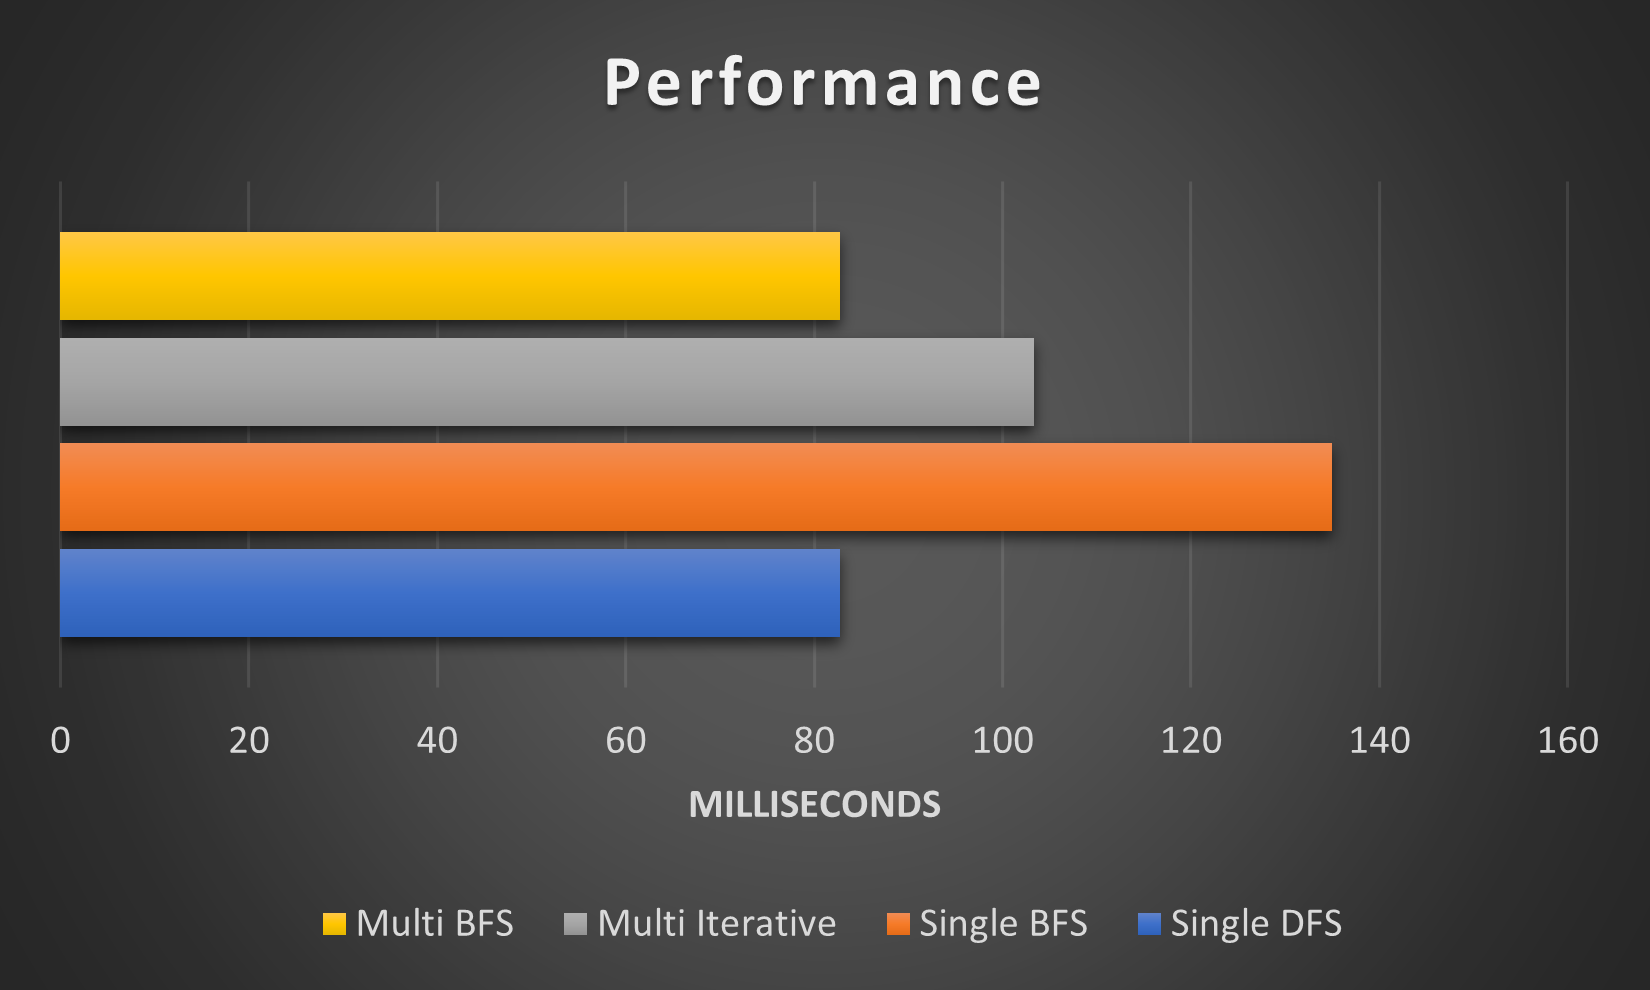
\includegraphics[width=8cm,height=4.87cm]{Picture3.png}
\end{figure}
The performance of each program is displayed in the graph above this section. The Single Breadth First Search Memoization approach had an average performance time is 135 milliseconds, the Multi-threaded Iterative approach had an average performance of 103.333 milliseconds, and both the Single-threaded Depth First Search and Multi-threaded Breath First Search approaches had an average performance of 82.667 milliseconds on the machine we tested on.

\section{Discussion}
On some machines, the single threaded approach ran faster than the multi-threaded approach. We determined that the cause of this comes from two things:
\begin{enumerate}
    \item The puzzle complexity. The overhead of creating new threads on a processor that doesn't have many cores may not be worth it for a simpler puzzle.
    \item The computer's processor. For very complex puzzles with multiple solutions, a multi-threaded approach may be more efficent than the single threaded approach. Thus some devices that we had tested on that had faster processors with more cores were able to find the multiple solutions to a Sudoku puzzle much faster than the single threaded approach.
\end{enumerate}

\section{Conclusion}
The conclusions we reached from this project are that: 
\begin{enumerate}
\item Multithreading approaches support multiple solutions successfully
\item In brute force implementations, depth first searches algorithms outcompete breadth first search algorithms.
A multithreaded breadth first search is either the same speed or slower than a single threaded depth first search
\item Multithreading a brute force implementation doesn’t necessarily speed up solving sudoku puzzles because of the intent in the game.
Since only certain numbers work in a given position of the puzzle, all possible puzzle states are limited and diminish the purpose in brute force
\item Algorithmic strategies take the cake in famous sudoku solving algorithms such as “Dancing Links” and “Simulated Annealing” that are handcrafted for solving Sudoku Puzzles
\end{enumerate}


\section*{References}

\vspace{1\baselineskip}
[1] McGuire, Gary, et al. “There Is No 16-Clue Sudoku: Solving the Sudoku Minimum Number of Clues Problem.” NASA/ADS, https://ui.adsabs.harvard.edu/abs/2012arXiv1201.0749M
/abstract. 


\printbibliography


\end{document}
